\documentclass{./../../Latex/homework}
\begin{document}
\thispagestyle{plain}
\myheader{Homework 8 Solutions}

%%%%%%%%%%%%%% Exercise 9.2
\subsection*{Exercise 9.2} 

\begin{enumerate}
% Question 1
\item[1.] (c) $y=3 x^{2}+3$
$$ \quad \frac{d y}{d x}=6 x=0 \rightarrow x^{*}=0 $$
In the immediate neighborhood of $0$, for $x<0, \frac{d y}{d x}<0$, while for $x>0, \frac{d y}{d x}>0$. This implies that at $0$, the slope of the function changes sign from negative to positive i.e. the function was decreasing on the left of 0 but is increasing on the right. So it must be that the function has a relative minimum ($f(0)=3$) at $x=0$. We can also confirm this by looking at the 2nd derivative: $$\frac{d^{2} y}{d x^{2}}=6>0$$ \\
The graph of this function is given below: \\

\begin{center}
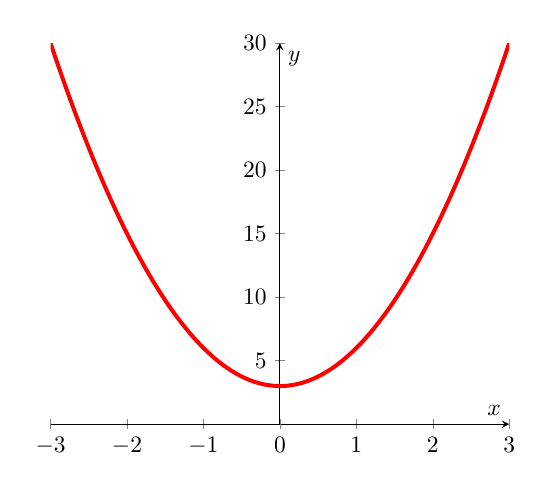
\begin{tikzpicture}[scale=0.85, transform shape]
\begin{axis}[axis lines = center, xlabel = \(x\), ylabel = \(y\), ytick distance=5, xtick distance=1, extra x ticks = {0}, ymin=0]
\addplot [domain=-3:3, samples=100, color=red, line width = 0.6mm]
{3*x^2+3};
\end{axis}
\end{tikzpicture}
\end{center}

% Question 2
\newpage
\item[2.] 
 (a) $y=x^{3}-3 x+5$

$$\frac{d y}{d x}=3 x^{2}-3=0 \rightarrow x^{*}= \pm \sqrt{1}$$ \\
So, we have two critical values $x_{1}^{*}=1$ and $x_{2}^{*}=-1$. \\

The derivative of the function, $3\left(x^{2}-1\right)$, is negative on the immediate left of 1 (e.g. $0.9$) and is positive on the immediate right of 1 (e.g. 1.1). While it is positive on the immediate left of $-1$ (e.g. -1.1) but negative on the right (e.g. -0.9). So the function should have a relative minimum at 1 and a relative maximum at -1. However, the domain of this function is limited to positive real numbers, in which case $-1$ is not permissible. So we only have a relative minimum $f(1)=3$.  \\

The graph (solid line) of this function is given below:

\begin{center}
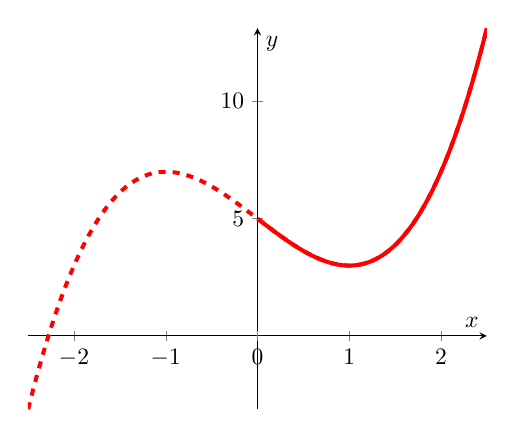
\begin{tikzpicture}[scale=0.85, transform shape]
\begin{axis}[axis lines = center, xlabel = \(x\), ylabel = \(y\), ytick distance=5, xtick distance=1, extra x ticks = {0}]
\addplot [domain=0:2.5, samples=100, color=red, line width = 0.6mm]
{x^3-3*x+5};
\addplot [domain=-2.5:2.5, samples=100, color=red, line width = 0.6mm, style=dashed]
{x^3-3*x+5};
\end{axis}
\end{tikzpicture}
\end{center}

We could have also reached the above conclusion from the second derivative test.
$$
\frac{d^{2} y}{d x^{2}}=6 x
$$
$\frac{d^{2} y}{d x^{2}}>1$ when $x=1 \rightarrow 1$ relative minimum at 1

$\frac{d^{2} y}{d x^{2}}<0$ when $x=-1 \rightarrow-1$ relative maximum at -1

\newpage

% Question 3
\item[3.] $f(x)=x+\frac{1}{x}$
$$
f^{\prime}(x)=1-\frac{1}{x^{2}}=0 \rightarrow x^*=\pm 1
$$
The derivative of the function, $(x^2-1)/x^2$, is negative on the immediate left of 1 (e.g. $0.9$) and is positive on the immediate right of 1 (e.g. 1.1). While it is positive on the immediate left of $-1$ (e.g. -1.1) but negative on the right (e.g. -0.9). So the function should have a relative minimum at 1 and a relative maximum at -1.

$$
\begin{aligned}
& f(1)=2 \\
& f(-1)=-2
\end{aligned}
$$
Here, the relative maximum $f(-1)=0$ is lower than the relative minimum $f(1)=2$. However, it is still correct as these are just \textit{relative} extrema. The graph for this function clarifies this notion. \\

\begin{center}
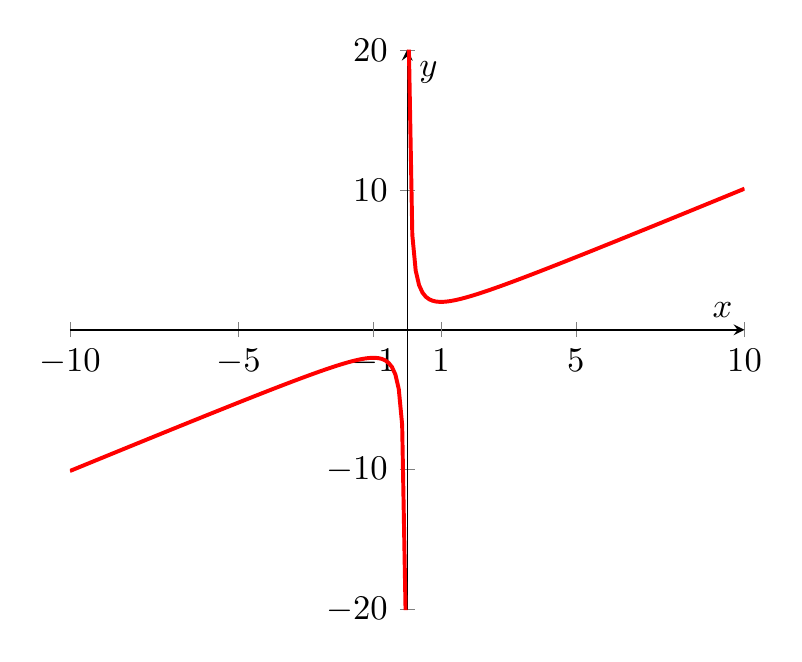
\begin{tikzpicture}[scale=1.25, transform shape]
\begin{axis}[axis lines = center, xlabel = \(x\), ylabel = \(y\), xtick distance=5, extra x ticks = {-1,1}]
\addplot [domain=0.05:10, samples=100, color=red, line width = 0.4mm]{x+(1/x)};
\addplot [domain=-10:-0.05, samples=100, color=red, line width = 0.4mm]{x+(1/x)};
\end{axis}
\end{tikzpicture}
\end{center}

\newpage

% Question 4
\item[4.] $T=\phi(x)$
\begin{enumerate}
  \item[(a)] $M=\phi^{\prime}(x)$
  \item[(b)] $A=\phi(x)/x$
  \item[(c)] Critical point:
  $$A^{\prime}=\frac{\phi^{\prime}(x) x-\phi(x)}{x^{2}}=0 \rightarrow \phi^{\prime}(x^*)=\frac{\phi(x^*)}{x^*}$$
  \item[(d)] Elasticity of $T$: $$\varepsilon=\frac{\phi^{\prime}(x) x}{\phi(x)}=\frac{M}{A}$$
  When $M=A \rightarrow \varepsilon=1$ \\~\\
\end{enumerate}
\end{enumerate}

%%%%%%%%%%%%%% Exercise 9.3
\subsection*{Exercise 9.3} 

\begin{enumerate}
% Question 2
\item[2.]
\begin{enumerate}

\item[(a)] $f(x)=9 x^{2}-4 x+8$
$$
\begin{aligned}
&f^{\prime}(x)=18 x-4 \\
&f^{\prime \prime}(x)=18>0 \\
\end{aligned}
$$
The function is strictly convex. \\

\item[(b)]$w=-3 x^{2}+39$
$$
\begin{aligned}
&\frac{d w}{d x}=-6 x \\
&\frac{d^{2} w}{d x^{2}}=-6<0
\end{aligned}
$$
The function is strictly concave. \\

\item[(c)]$u=9-2 x^{2}$
$$
\begin{aligned}
&f^{\prime}(x)=-4 x \\
&f^{\prime \prime}(x)=-4<0 \\
\end{aligned}
$$
The function is strictly concave. \\

\item[(d)]$v=8-5 x+x^{2}$
$$
\begin{aligned}
&\frac{d v}{d x}=-5+2 x
\end{aligned}
$$
$$
\frac{d^{2} v}{d x^{2}}=2>0
$$
The function is strictly convex.

\end{enumerate}

% Question 3
\item[3.] 
\begin{enumerate}
\item Concave but not strictly concave
\begin{center}
\begin{tikzpicture}[scale=0.75, transform shape]
\begin{axis}[axis lines = center, xlabel = \(x\), ylabel = \(y\), ytick distance=1, xtick distance=11, extra x ticks = {0}, ymax=3]
\addplot [domain=0:4, samples=100, color=red, line width = 0.6mm]{x^0.5};
\addplot [domain=4:10, samples=100, color=red, line width = 0.6mm]{2};
\end{axis}
\end{tikzpicture}
\end{center}
\item Concave and convex
\begin{center}
\begin{tikzpicture}[scale=0.75, transform shape]
\begin{axis}[axis lines = center, xlabel = \(x\), ylabel = \(y\), ytick distance=1, xtick distance=11, extra x ticks = {0}, ymax=3]
\addplot [domain=0:4, samples=100, color=red, line width = 0.6mm]{x};
\end{axis}
\end{tikzpicture}
\end{center}
\end{enumerate}


%\includegraphics[max width=\textwidth]{2022_10_30_958fe91d2cb3b80dda2bg-5}

% Question 4
\item[4.] We are given the following function:$$\quad y=a-\frac{b}{c+x} \quad(a, b, c>0, x \geqslant 0)$$

\begin{enumerate}
\item $$\frac{d y}{d x}=\frac{b}{(c+x)^{2}}>0$$

$$\frac{d^{2} y}{d x^{2}}=\frac{-b}{(c+x)^{4}} \cdot 2(c+x)$$

$$=\frac{-2 b}{(c+x)^{3}}<0$$ 
\item When $x=0$, $$y=a-\frac{b}{c}$$

\item As $x \rightarrow \infty, y \rightarrow a$ \\

We should restrict $a c>b$ to ensure consumption is positive. We should also make sure consumption  ($y$) does not increase more than one-to-one with income ($x$), such that $dy/dx < 1$, so $b<c^2$.   \\
\end{enumerate}

%\includegraphics[max width=\textwidth]{2022_10_30_958fe91d2cb3b80dda2bg-6}

% Question 5
\item[5.]
\begin{center}
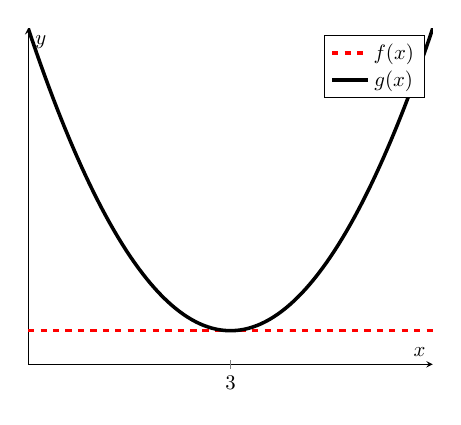
\begin{tikzpicture}[scale=0.75, transform shape]
\begin{axis}[axis lines = center, xlabel = \(x\), ylabel = \(y\), ytick distance=11, xtick distance=11, extra x ticks = {3}, ymin=0]
\addplot [domain=0:6, samples=100, color=red, line width = 0.6mm, style=dashed]{1};
\addlegendentry{\(f(x)\)}
\addplot [domain=0:6, samples=100, color=black, line width = 0.6mm]{x^2-6*x+10};
\addlegendentry{\(g(x)\)}
\end{axis}
\end{tikzpicture}
\end{center} 
$f(x)$ has infinitely many stationary points, while $g(x)$ has one stationary point $3$. 
\end{enumerate}


%%%%%%%%%%%%%% Exercise 9.4
\subsection*{Exercise 9.4} 

\begin{enumerate}
% Question 1	
\item[1.] (b)
$$
\begin{aligned}
f(x) &=x^{3}+6 x^{2}+9 \\
f^{\prime}(x) &=3 x^{2}+12 x \\
&=3 x(x+4) \rightarrow x^{*}=0,-4 \\
f^{\prime \prime}(x) &=6 x+12 \\
f^{\prime \prime}(0) &=12>0 \rightarrow f(0)=9 \text { is a local min } \\
f^{\prime \prime}(-4) &=-24+12=-12 \rightarrow f(-4) = 41 \text { is a local max }
\end{aligned}
$$ \\

% Question 2
\item[2.]
$$
\begin{aligned}
&A=x y \\
&2 x+y=64 \rightarrow y=64-2 x \\
&A=x(64-2 x)=64 x-2 x^{2} \\
&\frac{d A}{d x}=64-4 x \rightarrow x^*=16
\end{aligned}
$$
To see if it is indeed the maximum:
$$
\frac{d^2 A}{d x^2}=-4 <0 
$$ \\

% Question 3
\item[3.]
\begin{enumerate}
\item Yes
\item
$$
\begin{aligned}
R = P Q &= (100-Q) Q \\
&=100 Q-Q^{2}
\end{aligned}
$$
\item $\pi=R-C$
$$
=100 Q-Q^{2}-\frac{1}{3} Q^{3}+7 Q^{2}-111 Q-50
$$
$$
\begin{aligned}
& =-\frac{1}{3} Q^{3}+6 Q^{2}-11 Q-50
\end{aligned}
$$
\item $\frac{d \pi}{d Q}=-Q^{2}+12 Q-11=0$
$$
Q^{2}-12 Q+11=0
$$
$$
\begin{aligned}
& Q^{2}-11 Q-Q+11=0 \\
& Q(Q-11)-1(Q-11)=0 \\
& (Q-1)(Q-11)=0 \rightarrow Q^{*}=1 \text { and } 11
\end{aligned}
$$
$$
\frac{d^{2} \pi}{d Q^{2}}=-2 Q+12
$$
At $Q=1,-2+12=10>0$

At $Q=11,-22+12=-10<0$, so profit maximizing $Q=11$. \\
\item
$$
\begin{aligned}
\pi=&-\frac{1}{3} Q^{3}+6 Q^{2}-11 Q-50 \\
=& Q\left[Q\left[-\frac{1}{3} Q+6\right]-11\right]-50 \\~\\
\operatorname{Max} \pi=& 11\left[11\left(6-\frac{11}{3}\right)-11\right]-50 \\
& 11\left(11 \times\left(\frac{7}{3}-1\right)\right]-50 =40.75 \\
\end{aligned}
$$ \\~\\
\end{enumerate}

% Question 5
\item[5.] Profit function:
$$ \pi(Q) = hQ^2+jQ+k  $$
\begin{enumerate}
  \item $\pi(0) = k<0$
  \item $\pi'(Q) = 2hQ+j$, $\quad \pi''(Q) = 2h<0 \rightarrow h<0$
  \item Critical point: $\pi'(Q) = 2hQ+j=0 \rightarrow Q^* = -j/2h$. Since we assumed $h<0$, assuming $j>0$ ensures $Q^*>0$. 
\end{enumerate}
\end{enumerate}


%\begin{tikzpicture}[scale=0.75, transform shape]
%\begin{axis}[axis lines = center, xlabel = \(x\), ylabel = \(f(x)\)]
%\addplot [domain=-1:1, samples=100, color=red, line width = 0.5mm]
%{x^2};
%\end{axis}
%\end{tikzpicture}


\end{document}